\section{Реализация, тестирование и демонстрация решателя задач}

\subsection{Выбор средств и технологий реализации}

Индивидуальная программная реализация выполнена в виде одностраничного клиентского приложения CoWo. Клиент предоставляет единое рабочее пространство для авторизации, загрузки документов, наблюдения за фоновой обработкой, просмотра карточек, исследования графа знаний и отправки вопросов. Агентное ядро и серверная инфраструктура не дублируются на стороне браузера: фронтенд получает их результаты через типизированные REST-контракты и отвечает за корректное представление состояний пользователю.

В качестве основной библиотеки выбран React~19.2. Компонентная модель React позволяет собирать интерфейс из изолированных частей с собственной логикой и представлением. \cite{ReactDocs2026} В реализации отдельными компонентами оформлены авторизация, зона загрузки, список документов, карточка знания, граф и экран вопроса. Состояние компонентов хранится с помощью хуков \texttt{useState}, а синхронизация с внешними данными и таймерами выполняется в \texttt{useEffect}.

Исходный код написан на TypeScript~5.7. TypeScript выполняет статическую проверку JavaScript-программ до их запуска и позволяет явно описывать отношения между данными. \cite{TypeScriptDocs2026} Для каждого ответа API определён отдельный тип: \texttt{User}, \texttt{Job}, \texttt{StoredJob}, \texttt{KnowledgeCard}, \texttt{KnowledgeGraph} и \texttt{Answer}. Это уменьшает риск несогласованности имён полей между сервером и визуальными компонентами.

Средой разработки и сборки служит Vite~6. В режиме разработки Vite предоставляет сервер с поддержкой модулей и быстрым обновлением, а команда производственной сборки формирует статический пакет, пригодный для размещения веб-сервером. \cite{ViteDocs2026} В проекте настроено проксирование пути \texttt{/api} на сервер приложения, поэтому клиент использует относительные URL и не хранит адрес API внутри компонентов.

Сетевое взаимодействие построено на стандартном браузерном Fetch API. Fetch предоставляет основанный на \texttt{Promise} интерфейс HTTP-запросов и возвращает объект \texttt{Response}, статус которого требуется проверять явно. \cite{FetchMDN2026} Для передачи файлов используется \texttt{FormData}; браузер самостоятельно формирует границу \texttt{multipart/form-data}, поэтому клиент не задаёт заголовок \texttt{Content-Type} вручную. \cite{FormDataMDN2026}

Граф визуализируется средствами встроенного SVG без тяжёлой внешней библиотеки раскладки. SVG поддерживает линии, текст, группы, трансформации и взаимодействие через DOM, что позволяет создавать интерактивную векторную сцену непосредственно в браузере. \cite{SVGMDN2026} Иконки берутся из набора \texttt{lucide-react}, а вся компоновка, цветовая схема, адаптивность и анимации описаны в собственном CSS.

Состав применённых средств приведён в таблице~\ref{tab:frontend_technologies}.

\begin{table}[h!]
\caption{Средства реализации клиентского приложения}
\label{tab:frontend_technologies}
\begin{tabularx}{\textwidth}{|X|X|X|}
\hline
\textbf{Средство} & \textbf{Назначение} & \textbf{Применение в проекте} \\
\hline
React~19.2 & Компонентное представление интерфейса & Экраны, локальное состояние, обработка событий \\
\hline
TypeScript~5.7 & Статическая типизация & API-контракты, свойства компонентов, состояния \\
\hline
Vite~6 & Разработка и сборка & Dev-сервер, proxy \texttt{/api}, production bundle \\
\hline
Fetch API & HTTP-взаимодействие & JSON-запросы, обновление токена, обработка ошибок \\
\hline
FormData, Blob & Работа с файлами & Пакетная загрузка и скачивание оригинала \\
\hline
SVG & Визуализация графа & Узлы, рёбра, области сообществ, панорамирование \\
\hline
Lucide React & Пиктограммы & Навигация, статусы, действия пользователя \\
\hline
CSS & Внешний вид и адаптивность & Сетка, модальные окна, breakpoints, reduced motion \\
\hline
Nginx & Публикация сборки & Статические файлы и проксирование API \\
\hline
\end{tabularx}
\end{table}

Выбранный стек не требует отдельного клиентского хранилища состояния и библиотеки построения графов. Для текущего объёма прототипа локального состояния React и детерминированной SVG-раскладки достаточно, а число производственных зависимостей остаётся небольшим.

\subsection{Структура программной реализации}

Исходный код клиентской части расположен в каталоге \texttt{frontend/src}. Точка входа \texttt{main.tsx} создаёт корневой React-узел и подключает глобальные стили. Компонент \texttt{App} выполняет роль координатора: восстанавливает пользовательскую сессию, загружает документы, переключает основные представления и открывает карточку в модальном окне. Специализированные компоненты не обращаются друг к другу напрямую, а получают данные и обработчики через свойства.

Структура основных модулей приведена в таблице~\ref{tab:frontend_modules}.

\begin{table}[h!]
\caption{Модули клиентской реализации}
\label{tab:frontend_modules}
\begin{tabularx}{\textwidth}{|X|X|X|}
\hline
\textbf{Файл} & \textbf{Ответственность} & \textbf{Основные данные} \\
\hline
\texttt{App.tsx} & Координация приложения и навигация & Пользователь, документы, уведомление, открытая карточка \\
\hline
\texttt{AuthScreen.tsx} & Вход и регистрация & Email, пароль, режим формы, ошибка \\
\hline
\texttt{UploadZone.tsx} & Выбор и отправка файлов & Список файлов, drag-and-drop, локальная проверка \\
\hline
\texttt{JobsTable.tsx} & Библиотека и статусы & Задания, этапы, действия просмотра и удаления \\
\hline
\texttt{CardModal.tsx} & Просмотр карточки & Summary, тезисы, домен, сообщество, концепции \\
\hline
\texttt{GraphExplorer.tsx} & Раскладка и навигация по графу & Сообщества, домены, концепции, рёбра, координаты \\
\hline
\texttt{AskPanel.tsx} & Вопрос и представление ответа & Текст вопроса, ответ, источники, пути \\
\hline
\texttt{lib/api.ts} & Единый HTTP-клиент & Access-токен, refresh-запрос, ошибки, методы API \\
\hline
\texttt{types.ts} & Контракты данных & Типы всех серверных ответов \\
\hline
\texttt{styles.css} & Визуальная система & Цвета, сетки, состояния, адаптивные правила \\
\hline
\end{tabularx}
\end{table}

Верхнеуровневое состояние навигации задаётся объединением строковых литералов. Такой тип исключает переход к несуществующему экрану на этапе компиляции:

\begin{verbatim}
type View = "library" | "graph" | "ask";

const [view, setView] = useState<View>("library");
const [jobs, setJobs] = useState<StoredJob[]>([]);
const [openCard, setOpenCard] = useState<OpenCard | null>(null);
\end{verbatim}

Основное рабочее пространство имеет три состояния. Экран \texttt{library} содержит показатели базы, загрузчик и список документов. Экран \texttt{graph} монтирует интерактивную карту знаний. Экран \texttt{ask} предоставляет форму вопроса и область результата. На широком экране переключатели расположены в левой боковой панели, а при ширине до 820 пикселей боковая панель заменяется фиксированной нижней навигацией.

Компонентная зависимость показана на рисунке~\ref{fig:frontend_components_implementation}.

\begin{figure}[h!]
\centering
\begin{tabular}{c}
\fbox{\parbox{0.72\textwidth}{\centering \texttt{main.tsx} $\rightarrow$ \texttt{App.tsx}}}\\[0.5em]
\begin{tabular}{c@{\hspace{0.5em}}c@{\hspace{0.5em}}c}
\fbox{\parbox{0.25\textwidth}{\centering \texttt{AuthScreen}}} &
\fbox{\parbox{0.25\textwidth}{\centering \texttt{Library}}} &
\fbox{\parbox{0.25\textwidth}{\centering \texttt{GraphExplorer}}} \\
& $\downarrow$ & \\
\fbox{\parbox{0.25\textwidth}{\centering \texttt{AskPanel}}} &
\fbox{\parbox{0.25\textwidth}{\centering \texttt{UploadZone}\\\texttt{JobsTable}}} &
\fbox{\parbox{0.25\textwidth}{\centering \texttt{CardModal}}}
\end{tabular}\\[0.5em]
\fbox{\parbox{0.72\textwidth}{\centering \texttt{api.ts} $+$ \texttt{types.ts} $+$ \texttt{styles.css}}}
\end{tabular}
\caption{Структура компонентов клиентского приложения}
\label{fig:frontend_components_implementation}
\end{figure}

Типы данных отделены от визуальных компонентов. Например, \texttt{KnowledgeCard} содержит служебные идентификаторы и объект \texttt{analysis}, включающий summary, массив ключевых положений, сообщество, домен и концепции. \texttt{KnowledgeGraph} содержит четыре независимых массива: сообщества, домены, концепции и рёбра. Компонент графа не предполагает фиксированного числа уровней и строит представление из этих массивов.

Стили организованы как единая визуальная система. В корневых CSS-переменных заданы основные цвета, границы и фон. Повторно используются классы панелей, кнопок, сообщений и индикаторов. Медиавыражения на 1100, 820 и 560 пикселях изменяют число колонок, переключают навигацию, упрощают строки документов и переводят карточку в одноколоночный режим. Отдельное правило \texttt{prefers-reduced-motion} практически отключает переходы и анимации для пользователя, выбравшего уменьшение движения в настройках системы.

\subsection{Реализация взаимодействия с базой знаний}

Клиент не обращается к PostgreSQL, MinIO или FalkorDB напрямую. Единственной точкой интеграции является модуль \texttt{lib/api.ts}, инкапсулирующий адреса маршрутов, сериализацию, токен доступа, обновление сессии и преобразование ошибок. Благодаря этому визуальные компоненты работают с предметными операциями: \texttt{listDocuments}, \texttt{getGraph}, \texttt{getCard}, \texttt{ask}, а не с деталями HTTP.

Базовая функция \texttt{rawRequest} создаёт объект заголовков и добавляет \texttt{Authorization}, если access-токен уже получен. Для JSON-тела устанавливается \texttt{Content-Type: application/json}; для \texttt{FormData} этот заголовок пропускается. Все запросы выполняются с \texttt{credentials: include}, чтобы браузер передавал HttpOnly cookie обновления сессии.

Если сервер отвечает кодом 401 не на маршруте авторизации, клиент один раз вызывает \texttt{refreshAccessToken} и повторяет исходный запрос. Одновременные запросы не создают несколько операций обновления: переменная \texttt{refreshRequest} хранит общий \texttt{Promise}, пока обновление не завершено. При ошибке токен удаляется из памяти, а пользователь возвращается к экрану входа при следующей проверке сессии.

Access-токен намеренно хранится в памяти модуля, а не в \texttt{localStorage}. После полной перезагрузки страницы приложение сначала обращается к маршруту обновления, затем получает текущего пользователя. Пока выполняется этот bootstrap, отображается отдельный экран загрузки; это предотвращает кратковременное появление формы входа у уже авторизованного пользователя.

Используемые маршруты перечислены в таблице~\ref{tab:frontend_api_routes}.

\begin{table}[h!]
\caption{Группы REST-маршрутов, используемые клиентом}
\label{tab:frontend_api_routes}
\begin{tabularx}{\textwidth}{|X|X|X|}
\hline
\textbf{Группа путей} & \textbf{Действия интерфейса} & \textbf{Результат} \\
\hline
\texttt{/auth/*} & Регистрация, вход, refresh, профиль и выход & Пользователь и токен \\
\hline
\texttt{/ingestion/documents*} & Загрузка и библиотека & Задания документов \\
\hline
\texttt{/ingestion/jobs/\{id\}*} & Статус, карточка, оригинал, повтор и удаление & Данные задания \\
\hline
\texttt{/graph*} & Граф и карточки выбранной концепции & Узлы, рёбра, карточки \\
\hline
\texttt{/retrieval/answer} & Отправка вопроса & Ответ, источники и пути \\
\hline
\end{tabularx}
\end{table}

Ошибки сервера преобразуются в пользовательские сообщения функцией \texttt{humanizeError}. В словаре предусмотрены отдельные тексты для неверных учётных данных, превышения размера файла, неподдерживаемого формата, отсутствия текста, тайм-аута разбора, отсутствия подходящего знания и незавершённой обработки. Если FastAPI возвращает массив ошибок валидации, клиент извлекает первое поле \texttt{msg}. Неизвестная строка ошибки выводится в читаемом виде после замены символов подчёркивания пробелами.

Скачивание оригинала также выполняется через общий механизм авторизации. Ответ преобразуется в \texttt{Blob}, для него создаётся временный \texttt{object URL}, после чего программно активируется элемент \texttt{a} с атрибутом \texttt{download}. Имя файла извлекается из \texttt{Content-Disposition}; при отсутствии заголовка используется имя из карточки или строки документа. После начала скачивания временный URL освобождается.

\subsection{Реализация пользовательских сценариев}

\subsubsection{Авторизация и восстановление сессии}

Экран \texttt{AuthScreen} объединяет режимы входа и регистрации. Переключение не создаёт новую страницу и очищает прежнюю ошибку. Поля используют стандартные типы \texttt{email} и \texttt{password}, атрибуты \texttt{required} и корректные значения \texttt{autocomplete}. Для регистрации до обращения к API проверяется минимальная длина пароля, наличие заглавной и строчной букв. Серверная проверка при этом остаётся обязательной и рассматривается как окончательная.

Во время отправки кнопка блокируется и содержит индикатор. Ошибка показывается как \texttt{role="alert"} с \texttt{aria-live="assertive"}, автоматически исчезает через шесть секунд и может быть закрыта вручную. После успешной регистрации клиент выполняет вход и повторно получает профиль, поэтому дальнейшее состояние совпадает для обоих режимов.

\subsubsection{Библиотека и загрузка документов}

Компонент \texttt{UploadZone} поддерживает выбор через системный диалог и drag-and-drop. Из входного списка оставляются PDF, DOCX, Markdown и TXT. Если часть файлов имеет другое расширение, пользователь видит предупреждение, но допустимые элементы сохраняются. Количество файлов в одном пакете ограничено десятью; перед отправкой отображаются имя и размер каждого файла, а отдельная кнопка позволяет удалить ошибочно выбранный элемент.

При отправке одного файла используется поле \texttt{file} и одиночный маршрут. Для двух и более файлов применяются поле \texttt{files} и batch-маршрут. Такой выбор скрыт внутри API-клиента, поэтому \texttt{UploadZone} всегда передаёт массив и не содержит условных URL.

После получения ответа созданные задания оптимистично добавляются в начало списка. Затем приложение пытается запросить полный список документов. Если повторное чтение временно недоступно, оптимистичные строки остаются на экране, а механизм опроса продолжает обновлять их по идентификаторам. Благодаря этому успешная загрузка не выглядит потерянной из-за сбоя вторичного запроса.

Список \texttt{JobsTable} отображает название, дату, номер попытки, этап и итоговый статус. Этапы сервера переводятся в понятные подписи: «Извлечение текста», «Разбиение», «Векторизация», «Анализ концептов» и «Запись графа». Для завершённого задания доступны карточка и скачивание, для ошибочного --- повтор, для queued и running --- индикатор обработки. Удаление не показывается для running-задания, чтобы действие интерфейса соответствовало серверному ограничению.

Перед удалением отображается стандартное подтверждение с именем документа. Идентификатор удаляемого задания добавляется в множество \texttt{deletingJobIds}; только соответствующая кнопка заменяется индикатором и блокируется. После ответа 204 строка удаляется из библиотеки, а открытая карточка этого же документа закрывается. Ошибка оставляет данные на месте и выводит уведомление.

Экран библиотеки с различными состояниями документов представлен на рисунке~\ref{fig:ui_library}.

\begin{figure}[h!]
\centering
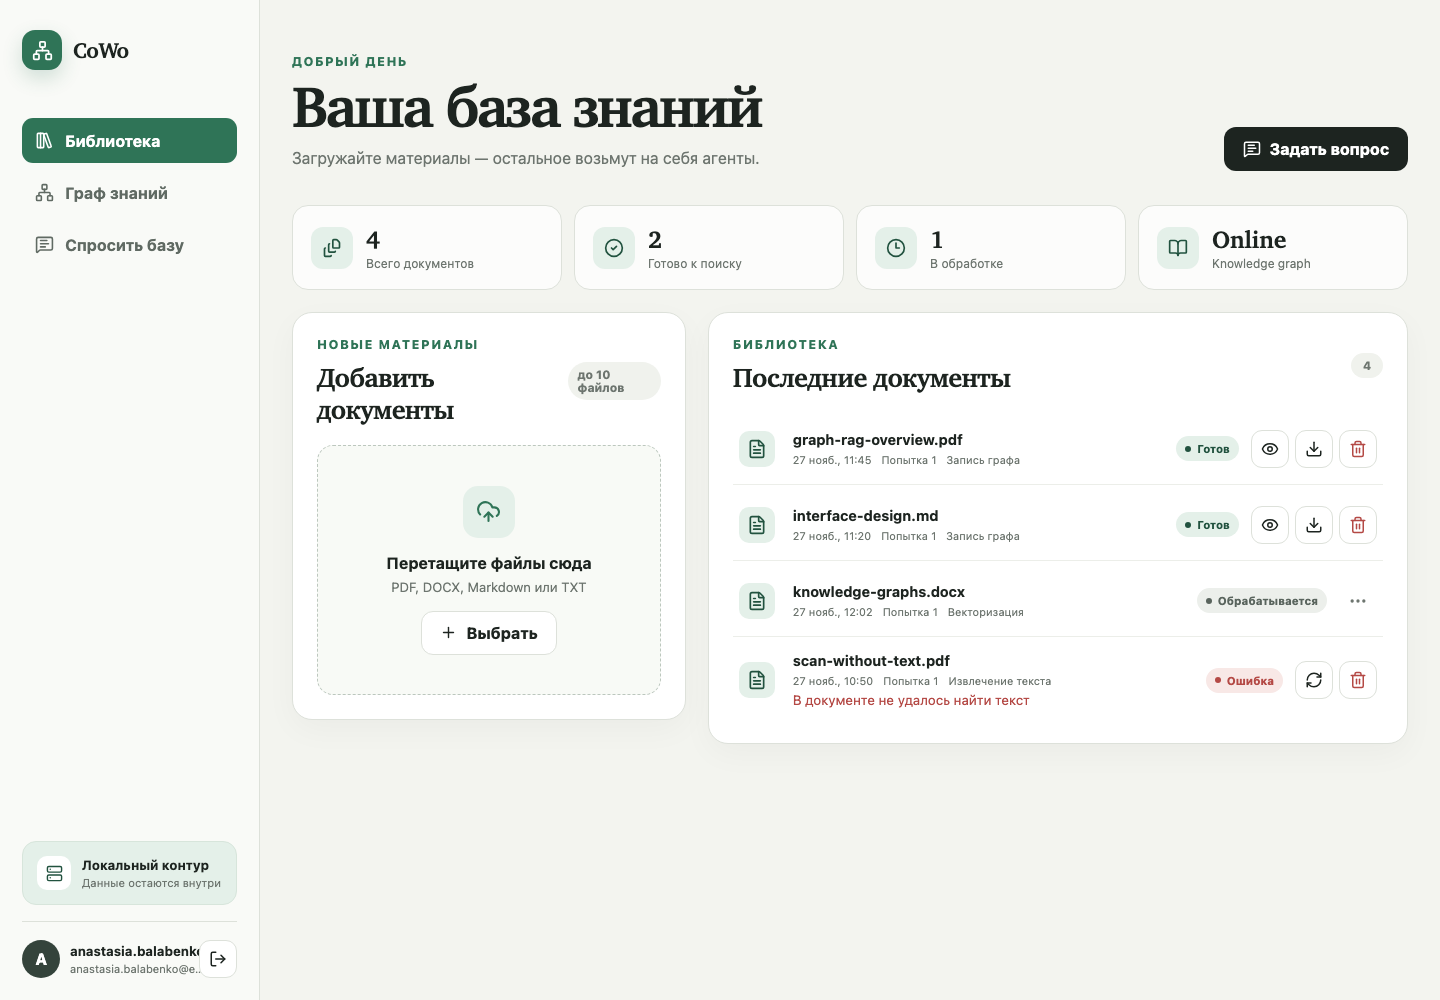
\includegraphics[width=\textwidth]{picture/ui_library.png}
\caption{Библиотека, загрузка документов и состояния обработки}
\label{fig:ui_library}
\end{figure}

\subsubsection{Обновление прогресса обработки}

Компонент \texttt{App} вычисляет строку идентификаторов заданий в состояниях \texttt{queued} и \texttt{running}. Если строка пуста, таймер не создаётся. В противном случае каждые 3,5 секунды запускается параллельное чтение состояний. Использование \texttt{Promise.allSettled} позволяет применить успешные ответы, даже если один из запросов завершился ошибкой.

Обновление выполняется функциональной формой \texttt{setJobs}, поэтому результат объединяется с последней версией массива, а не со снимком состояния на момент создания таймера. При изменении набора активных идентификаторов предыдущий интервал очищается функцией завершения эффекта. Когда все задания становятся completed, failed или cancelled, зависимость становится пустой и сетевой опрос прекращается.

Прогресс не интерпретируется как процент, поскольку продолжительность этапов неравномерна и зависит от документа и внешней модели. Вместо потенциально вводящей в заблуждение полосы отображаются дискретное состояние и текущий этап. Такое решение точно отражает доступный серверный контракт.

\subsubsection{Просмотр карточки знания}

Для завершённого документа карточка загружается только после действия пользователя. \texttt{CardModal} отображает имя исходного файла, аннотацию, домен, сообщество, ключевые мысли и концепции с описаниями. В нижней части расположены сокращённый идентификатор и действие скачивания оригинала.

Модальное окно закрывается кнопкой, нажатием на затемнённый фон или клавишей Escape. Событие мыши внутри карточки останавливает всплытие, поэтому взаимодействие с содержимым не приводит к случайному закрытию. Разметка использует \texttt{role="dialog"} и \texttt{aria-modal="true"}. При ширине до 560 пикселей пары домена и сообщества, а также сетка концепций переходят в одну колонку.

Один и тот же компонент карточки открывается из библиотеки и из графа. Для второго сценария данные карточки уже возвращены маршрутом концепции, а \texttt{App} формирует минимальный объект задания, необходимый для скачивания. Это устраняет дублирование визуального представления.

\subsubsection{Интерактивная визуализация графа}

После открытия экрана \texttt{GraphExplorer} один раз запрашивает полный пользовательский граф. До ответа показывается состояние загрузки, при пустом массиве концепций --- отдельное приглашение добавить первый документ, при ошибке --- локальное сообщение. Успешный ответ передаётся функции \texttt{buildLayout}, результат которой мемоизируется и пересчитывается только при изменении графа.

Каждому сообществу выделяется вертикальная область. Домены сообщества размещаются в сетке не более чем из двух колонок с ячейками $460 \times 390$ пикселей. Концепции домена располагаются кольцами по восемь элементов. Для концепции с номером $i$ номер кольца равен $\lfloor i/8 \rfloor$, угловая позиция определяется остатком $i \bmod 8$, а радиус вычисляется как
\begin{equation}
r_i = 138 + 76 \cdot \left\lfloor \frac{i}{8} \right\rfloor.
\end{equation}
Координаты доменов и концепций сохраняются в \texttt{Map}, что позволяет строить линии по идентификаторам без повторного поиска визуального элемента.

Области сообществ и все рёбра формируются SVG-элементами, а домены и концепции помещаются в \texttt{foreignObject}. Это позволяет использовать обычную HTML-разметку кнопок внутри векторной сцены. Межконцептуальные рёбра соединяют координаты source и target, доменные линии связывают концепцию с её доменом.

Пользователь может перемещать сцену указателем, изменять масштаб колесом или кнопками и возвращаться к исходному положению. Масштаб ограничен диапазоном от 0,48 до 1,35, что предотвращает исчезновение графа или чрезмерное увеличение. При выборе концепции она и непосредственные соседи выделяются, остальные узлы и рёбра приглушаются.

Наведение, клавиатурный фокус и нажатие на концепцию вызывают \texttt{revealCards}. Карточки загружаются только для выбранной концепции и сохраняются в словаре по идентификатору. Повторное наведение использует кэш. Всплывающая панель остаётся доступной для указателя и позволяет открыть полную карточку документа.

Результат визуализации показан на рисунке~\ref{fig:ui_graph}.

\begin{figure}[h!]
\centering
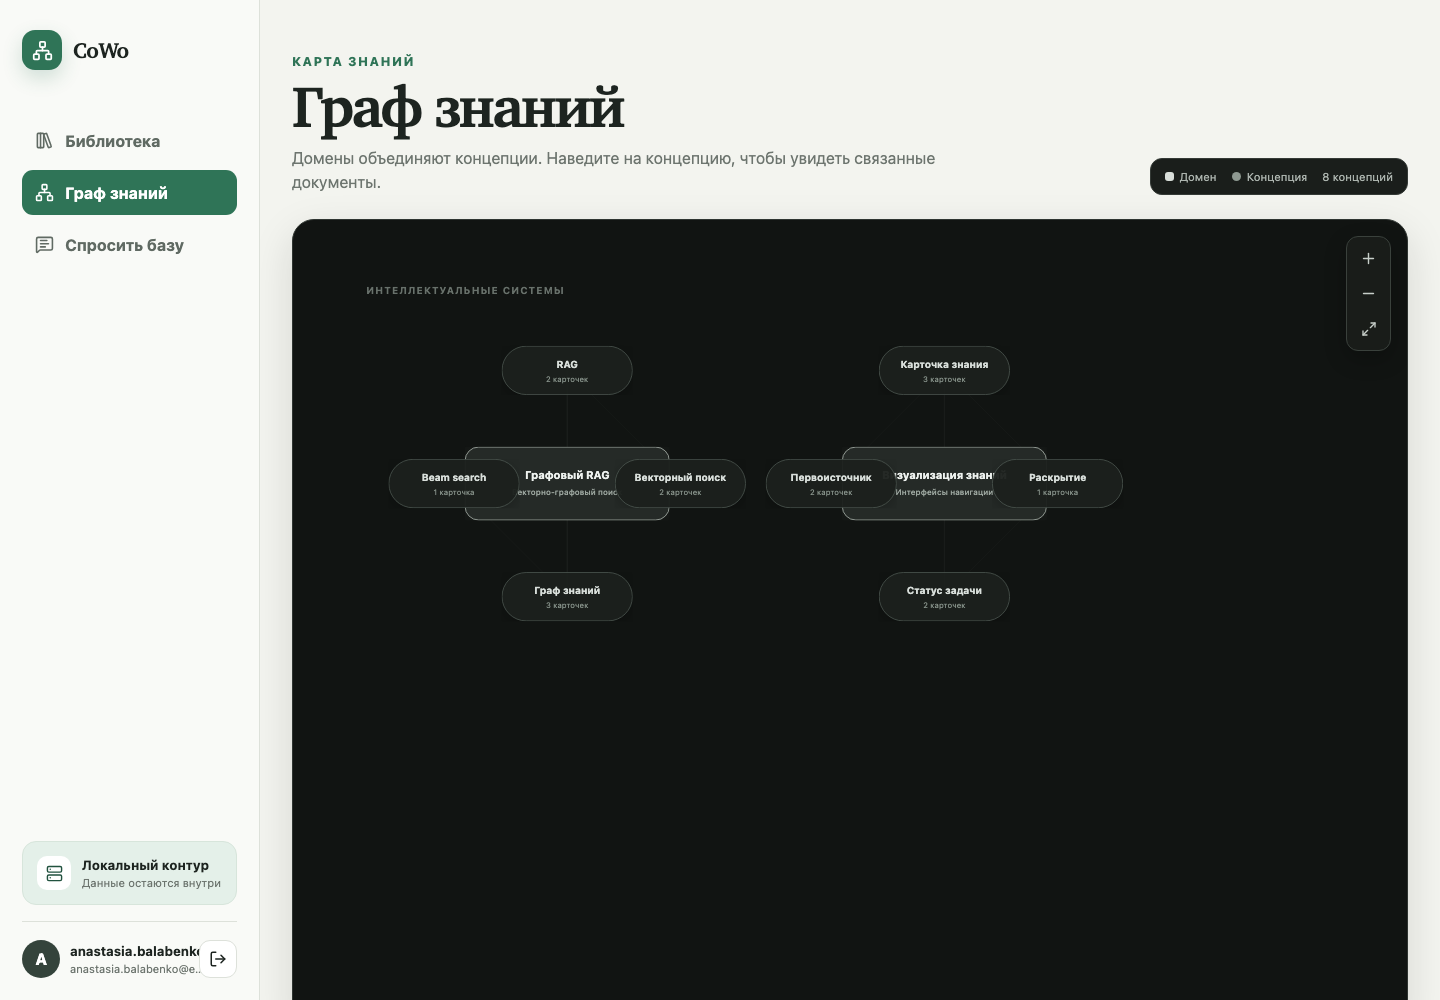
\includegraphics[width=\textwidth]{picture/ui_graph.png}
\caption{Интерактивная карта доменов, концепций и связей}
\label{fig:ui_graph}
\end{figure}

Текущая раскладка детерминирована и не использует физическую симуляцию. Это обеспечивает стабильное расположение между повторными открытиями одного графа и не создаёт постоянную нагрузку на процессор. Ограничением является рост размеров сцены при большом числе доменов и концепций; это учтено в направлениях дальнейшего развития.

\subsubsection{Диалог с базой знаний}

Компонент \texttt{AskPanel} хранит вопрос, ответ, состояние ожидания и ошибку. Пустая строка не отправляется, повторное действие во время запроса блокируется, длина ограничена 4000 символами. До первого ответа пользователь видит три примера вопросов, по нажатию выбранный текст переносится в поле.

Запрос отправляется в виде JSON-объекта \texttt{\{question\}}. Результат \texttt{Answer} включает текст, массив \texttt{citations} и массив \texttt{evidence\_paths}. Эти части намеренно отображаются отдельно: текст остаётся читаемым, источники имеют собственные кнопки скачивания, а путь представлен последовательностью концепций и процентом релевантности.

Каждый источник содержит идентификаторы карточки, задания, документа и версии, краткое содержание и авторизованный URL оригинала. Клиент не строит ссылку из пользовательского текста и не позволяет модели указать произвольный внешний адрес. Для скачивания используется тот же API-клиент с автоматическим обновлением токена.

Путь рассуждения выводится как упорядоченный набор меток. Если сервер возвращает несколько путей, каждый имеет собственный job ID и score. Клиент переводит значение score в целый процент только для представления, не изменяя порядок, вычисленный сервером.

Экран ответа приведён на рисунке~\ref{fig:ui_answer}.

\begin{figure}[h!]
\centering
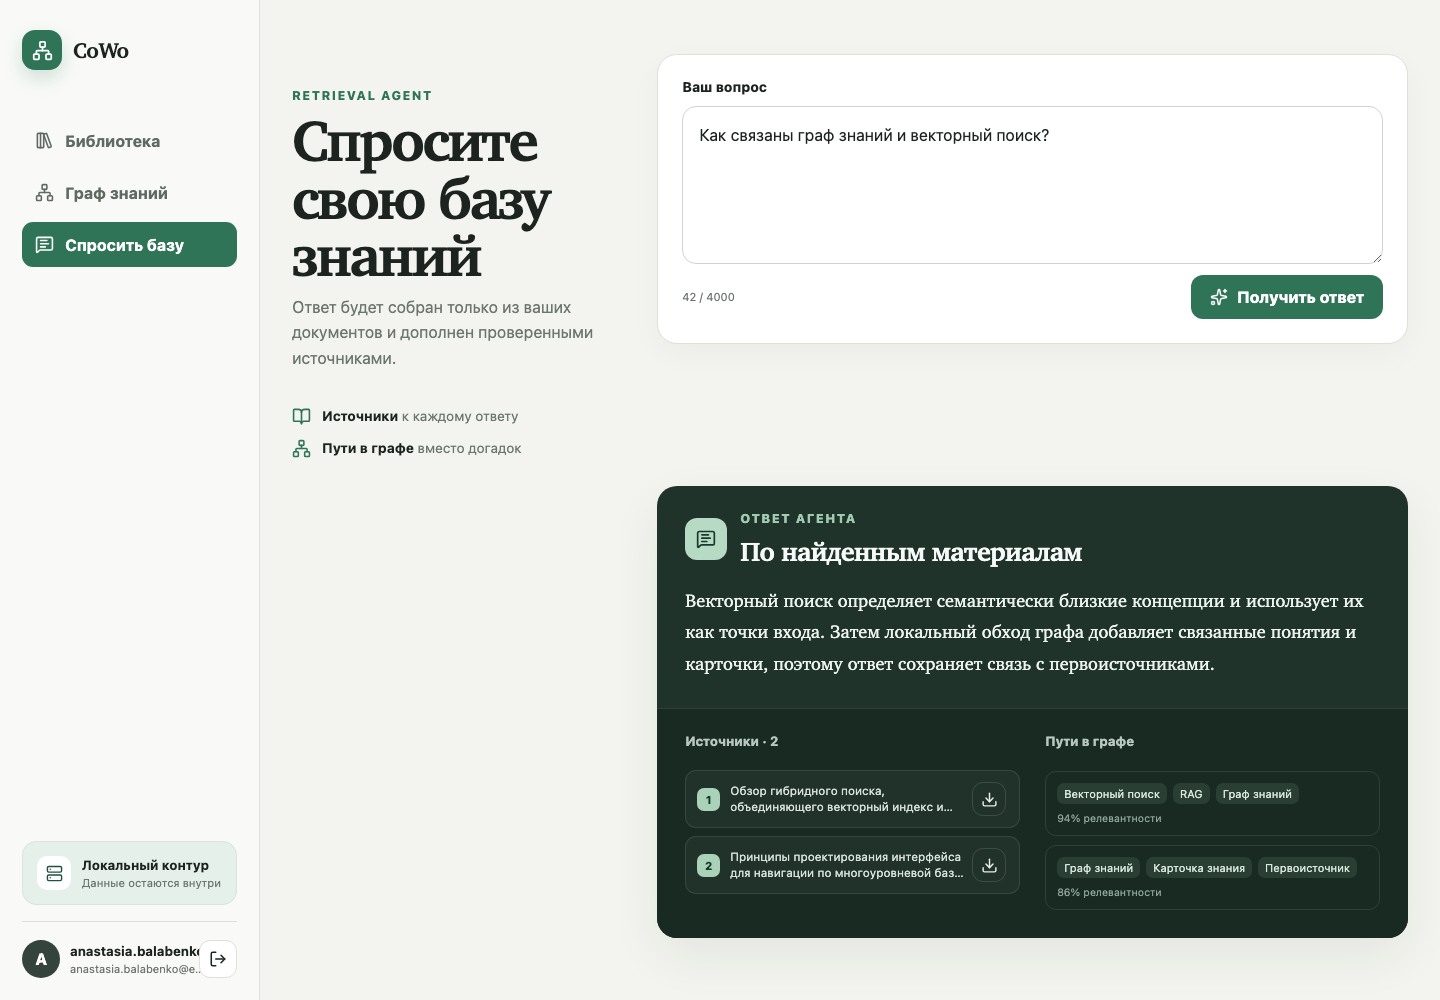
\includegraphics[width=\textwidth]{picture/ui_answer.png}
\caption{Ответ с подтверждающими источниками и путями в графе}
\label{fig:ui_answer}
\end{figure}

\subsection{Реализация доступности и адаптивного представления}

Интерфейс использует семантические элементы \texttt{main}, \texttt{nav}, \texttt{section}, \texttt{article}, \texttt{form}, \texttt{button} и \texttt{label}. Кнопки, содержащие только пиктограмму, снабжены \texttt{aria-label}; декоративные элементы экрана входа имеют \texttt{aria-hidden}. Поля связаны с подписями, а ошибочное поле пароля получает \texttt{aria-invalid}.

Сообщения об успехе используют \texttt{role="status"}, а ошибки ввода --- \texttt{role="alert"}. WCAG рекомендует программно определять сообщения о состоянии, чтобы вспомогательные технологии могли сообщить о результате без принудительного перевода фокуса. \cite{WCAG2026} Визуальный фокус задан для кнопок, полей и текстовой области через \texttt{:focus-visible}.

Дополнительная информация о концепции доступна не только по наведению, но также по фокусу и нажатию. Это позволяет взаимодействовать с узлами клавиатурой и на сенсорном устройстве. Модальная карточка закрывается Escape, а анимации учитывают системный режим reduced motion.

На экранах до 820 пикселей скрывается боковая панель и появляется нижняя навигация из трёх пунктов. Рабочая область занимает всю ширину, блоки вопроса и ответа переходят в одну колонку, а высота графа вычисляется относительно viewport. На экранах до 560 пикселей сокращается вторичная информация в строках документов, уменьшаются отступы и перестраиваются карточки. В результате сохраняются основные действия без горизонтального прокручивания всей страницы.

\subsection{Реализация обработки ошибок и граничных состояний}

Для каждого основного экрана предусмотрены состояния loading, empty, success и error. При инициализации приложения показывается экран загрузки; при отсутствии пользователя --- авторизация; при пустой библиотеке --- приглашение добавить документ; при пустом графе --- объяснение, почему узлы отсутствуют. Такой подход исключает пустые белые области, смысл которых пользователь должен угадывать.

Клиент различает локальную и серверную валидацию. Локально проверяются очевидные условия, не требующие сети: расширение, количество файлов, непустой вопрос и базовая политика пароля. Ограничения размера, содержимого, владельца и состояния задания проверяет сервер. Ответ сервера всегда обрабатывается, даже если клиентская проверка была пройдена.

При пакетной загрузке ошибка не очищает выбранные файлы, поэтому пользователь может повторить действие. После успешной отправки список очищается и системное значение file input сбрасывается. При ошибке открытия карточки, скачивания, повтора или удаления текущий экран не заменяется: сообщение выводится в toast, а существующие данные сохраняются.

Опрос статусов использует частичный успех. Если один job временно недоступен, остальные обновляются, а прежнее состояние проблемного задания остаётся видимым. Сетевой сбой экрана графа отображается внутри рабочей области, не завершает сессию и не влияет на библиотеку.

Все временные эффекты имеют очистку. Таймер уведомления удаляется при замене сообщения, интервал опроса --- при изменении активных заданий, обработчик Escape --- при закрытии карточки. Это предотвращает обновление размонтированных компонентов и накопление обработчиков при переключении экранов.

\subsection{Тестирование сценариев работы решателя задач}

Тестирование индивидуальной части разделено на статическую проверку TypeScript, производственную сборку и ручные сценарии взаимодействия с API. Автоматические компонентные тесты в текущей версии фронтенда не подключены, поэтому в записке они не заявляются как выполненные. Команда \texttt{npm run build} последовательно запускает \texttt{tsc --noEmit} и \texttt{vite build}; контрольный запуск завершён без ошибок.

Сценарии ручного тестирования приведены в таблице~\ref{tab:frontend_tests}.

\begin{table}[h!]
\caption{Проверка пользовательских сценариев}
\label{tab:frontend_tests}
\begin{tabularx}{\textwidth}{|p{0.06\textwidth}|X|X|p{0.14\textwidth}|}
\hline
\textbf{№} & \textbf{Сценарий} & \textbf{Ожидаемый результат} & \textbf{Результат} \\
\hline
1 & Вход, регистрация и восстановление сессии & Открывается библиотека либо понятная ошибка & Соответствует \\
\hline
2 & Одиночная и пакетная загрузка & Создаются и отображаются задания & Соответствует \\
\hline
3 & Неверный формат или более десяти файлов & Применяется ограничение и предупреждение & Соответствует \\
\hline
4 & Обновление queued и running & Статус изменяется без перезагрузки & Соответствует \\
\hline
5 & Ошибка и повтор обработки & Показаны причина и действие повтора & Соответствует \\
\hline
6 & Карточка, оригинал и удаление & Действия относятся к выбранному документу & Соответствует \\
\hline
7 & Открытие, масштабирование и перемещение графа & Видны уровни и связи, viewport изменяется & Соответствует \\
\hline
8 & Выбор концепции & Выделяются соседи и связанные карточки & Соответствует \\
\hline
9 & Отправка вопроса & Выводятся ответ, источники и пути & Соответствует \\
\hline
10 & Узкий экран & Включается мобильная навигация & Соответствует \\
\hline
\end{tabularx}
\end{table}

Отдельно проверены негативные состояния: отсутствие документов, пустой граф, недоступность маршрута графа, ошибка ответа, сбой скачивания и отказ удаления выполняемого документа. Во всех случаях ранее загруженные данные не исчезают, а пользователь получает локальное сообщение без перезагрузки страницы.

Для демонстрационных снимков интерфейс запускался с контролируемыми ответами API, соответствующими рабочим TypeScript-контрактам. Это позволило воспроизводимо показать completed, running и failed документы, структуру графа и ответ с двумя источниками без зависимости от времени работы внешней языковой модели.

\subsection{Оценка качества и эффективности реализации}

Корректность клиентской реализации обеспечивается сочетанием статических типов, централизованного API-клиента и явных состояний компонентов. Типы фиксируют обязательные поля, единая функция запросов одинаково обрабатывает 401 и ошибки валидации, а визуальные компоненты не содержат собственных вариантов сетевого протокола.

Полнота индивидуальной реализации оценивается относительно пользовательских задач. Реализованы авторизация, загрузка одного файла и пакета, библиотека со статусами, повтор обработки, просмотр карточки, получение оригинала, удаление документа, визуализация графа, раскрытие связанных карточек, вопрос к базе, источники и пути рассуждения. Ручное объединение дубликатов и просмотр серверных логов относились к опциональному административному интерфейсу и в прототип не включены.

Эффективность сетевого взаимодействия обеспечивается тем, что опрос выполняется только для активных заданий и прекращается после достижения конечного состояния. Карточка загружается по требованию, а карточки концепции кэшируются на время жизни экрана графа. Параллельный опрос нескольких заданий не блокируется единичной ошибкой.

Производственная сборка сформировала JavaScript-файл размером около 237~КБ и CSS-файл размером около 28~КБ до gzip-сжатия. Внешняя библиотека физической раскладки графа отсутствует, поэтому вес клиента определяется главным образом React, иконками и прикладным кодом. Сформированные Vite файлы могут раздаваться как статические ресурсы через Nginx.

Визуальная устойчивость достигается стабильной компоновкой и ограничением размеров. Детерминированная раскладка не меняется после каждого взаимодействия, масштаб ограничен, длинные названия сокращаются многоточием, а прокручиваемая панель связанных карточек не расширяет SVG-сцену.

Доступность реализована частично: присутствуют семантические элементы, названия кнопок, статусы, видимый фокус, клавиатурное открытие концепций и reduced motion. Ограничением остаётся отсутствие полного управления фокусом внутри модального окна и специальной клавиатурной навигации между узлами SVG. Эти элементы включены в направления развития.

\subsection{Демонстрация работы решателя задач}

Демонстрация начинается с входа пользователя. После восстановления сессии открывается библиотека, где видны общее число документов, число завершённых и обрабатываемых заданий. Пользователь переносит PDF, DOCX, Markdown или TXT в область загрузки, проверяет список и отправляет пакет.

Новая строка появляется сразу после принятия запроса. По мере выполнения обновляются статус и этап. Завершённый документ открывается в карточке; из неё можно скачать оригинал. Для ошибочного документа доступен повтор, а удаление требует подтверждения и после успеха убирает документ из текущего состояния интерфейса.

На следующем этапе пользователь открывает граф знаний. Сообщества образуют области, домены расположены внутри них, а концепции сгруппированы вокруг доменов. Масштаб и положение сцены изменяются без перезагрузки. Выбор концепции выделяет непосредственные связи и показывает список карточек; выбранная карточка открывается в том же модальном представлении, что и из библиотеки.

Затем пользователь переходит на экран вопроса, выбирает подсказку или вводит собственный текст. После получения результата интерфейс показывает ответ, подтверждающие документы и пути по концепциям. Кнопка источника загружает оригинал через авторизованный маршрут. Таким образом, демонстрация проходит полный путь от добавления материала до навигации и проверяемого ответа.

Последовательность демонстрации приведена на рисунке~\ref{fig:frontend_demo_flow}.

\begin{figure}[h!]
\centering
\begin{tabular}{c@{\hspace{0.35em}$\rightarrow$\hspace{0.35em}}c@{\hspace{0.35em}$\rightarrow$\hspace{0.35em}}c}
\fbox{\parbox{0.22\textwidth}{\centering Вход и\\библиотека}} &
\fbox{\parbox{0.22\textwidth}{\centering Загрузка и\\статусы}} &
\fbox{\parbox{0.22\textwidth}{\centering Карточка и\\оригинал}}
\end{tabular}
\\[0.8em]
\begin{tabular}{c@{\hspace{0.5em}$\rightarrow$\hspace{0.5em}}c@{\hspace{0.5em}$\rightarrow$\hspace{0.5em}}c}
\fbox{\parbox{0.22\textwidth}{\centering Граф и\\концепции}} &
\fbox{\parbox{0.22\textwidth}{\centering Вопрос к\\базе}} &
\fbox{\parbox{0.22\textwidth}{\centering Ответ, источники\\и пути}}
\end{tabular}
\caption{Последовательность демонстрации клиентской подсистемы}
\label{fig:frontend_demo_flow}
\end{figure}

\subsection{Анализ ограничений и направления развития}

Первое ограничение связано с масштабом визуализируемого графа. Текущая версия получает все доступные пользователю узлы и рёбра и формирует SVG целиком. При тысячах концепций возрастут размеры DOM и стоимость выделения соседей. Развитием станет загрузка графа по сообществам и доменам, виртуализация элементов и индекс смежности вместо полного просмотра массива рёбер.

Второе ограничение --- отсутствие реализованных фильтров по сообществам и доменам. Иерархия уже отражается пространственным группированием, однако пользователь не может скрыть остальные группы. Следующим этапом является панель фильтров, поиск концепции и автоматическое центрирование выбранного узла.

Третье ограничение касается пути рассуждения. Сейчас путь отображается в ответе как последовательность меток, но не переносится на основной граф. Для полного выполнения расширенного сценария требуется передавать идентификаторы концепций, сохранять путь в общем состоянии и подсвечивать соответствующие узлы и рёбра в \texttt{GraphExplorer}.

Четвёртое ограничение относится к тестированию. Статическая проверка и ручные сценарии подтверждают работоспособность прототипа, но не заменяют регрессионные компонентные тесты. Планируется подключить Vitest и Testing Library для форм и состояний, а также Playwright для сквозных сценариев входа, загрузки, просмотра графа и вопроса.

Пятое ограничение связано с доступностью модального окна и графа. Необходимо реализовать focus trap, возврат фокуса на инициирующий элемент, объявление заголовка диалога через \texttt{aria-labelledby} и клавиатурное перемещение между соседними концепциями. Для графа также полезно предоставить альтернативное табличное представление.

Шестое ограничение --- периодический polling. Он прост и устойчив для прототипа, но создаёт запросы даже при отсутствии изменения этапа. В дальнейшем статусы можно передавать через Server-Sent Events или WebSocket, сохранив polling как резервный механизм.

Приоритетными направлениями развития являются фильтрация и поиск по графу, подсветка пути ответа на карте, автоматические тесты, улучшение доступности, потоковое обновление статусов и постраничная загрузка библиотеки.

\subsection{Выводы}

Реализовано клиентское веб-приложение для полного пользовательского цикла работы с базой знаний. Интерфейс поддерживает авторизацию, загрузку документов, отображение фоновых состояний, повтор, скачивание и удаление, просмотр карточек, визуальную навигацию по графу и получение ответа с источниками.

Разработан единый типизированный API-клиент с восстановлением сессии, переводом ошибок и безопасной работой с файлами. Реализована детерминированная SVG-раскладка сообществ, доменов и концепций, панорамирование, масштабирование, выделение связей и отложенная загрузка карточек.

Корректность подтверждена статической проверкой TypeScript, успешной производственной сборкой и ручным прохождением основных и ошибочных сценариев. Определены фактические ограничения прототипа и направления дальнейшего развития без приписывания клиентской части функций агентного ядра и серверной инфраструктуры.
